\documentclass{math}

\title{University Physics 1A}
\author{Alvin Lin}
\date{October 23rd, 2017}

\usepackage{tikz}

\begin{document}

\maketitle

\section*{Gravitational Force}
\[ F = \frac{Gm_1m_2}{R^2} \]
\[ U_g = -\frac{Gm_1m_2}{r} \]
At what point between the Earth and the Moon will a particle experience the
same force of gravitational attraction towards both bodies?
\begin{center}
  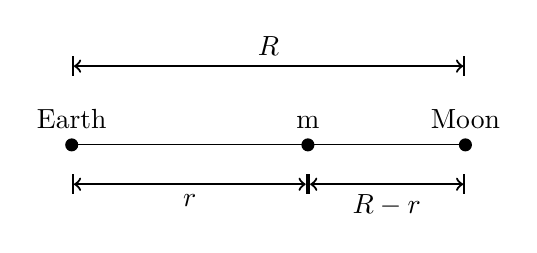
\begin{tikzpicture}
    \draw[|<->|,thick] (-2,1) -- (3,1) node[above,pos=0.5] {\( R \)};
    \draw (-2,0) node[circle,fill,scale=0.5,label=above:Earth]{} -- (1,0)
      node[circle,fill,scale=0.5,label=above:m]{} -- (3,0)
      node[circle,fill,scale=0.5,label=above:Moon]{};
    \draw[|<->|,thick] (-2,-0.5) -- (1,-0.5) node[below,pos=0.5] {\( r \)};
    \draw[|<->|,thick] (1,-0.5) -- (3,-0.5) node[below,pos=0.5] {\( R-r \)};
  \end{tikzpicture}
\end{center}
\begin{align*}
  F_{Earth} &= F_{Moon} \\
  G\frac{m_Em}{r^2} &= G\frac{m_{Moon}m}{(R-r)^2} \\
  \frac{(R-r)^2}{r^2} &= \frac{m_{Moon}}{m_{Earth}} \\
  \frac{R-r}{r} &= \pm\sqrt{m_{Moon}}{m_{Earth}} \\
  r &= 3.43\times10^5 km \\
  r &= 4.27\times10^4 km
\end{align*}

\subsection*{Escape Velocity}
Escape speed, \( v_{esc} \) (escape velocity) is defined as the speed with which
an object must be launched from the surface of a massive body (such as a planet)
so that it just barely escapes the planet (neglecting any air resistance). Find
the speed at which a mass \( m \) needs to be launched in order to escape the
gravity of a planet of size \( R \).
\begin{center}
  \begin{tikzpicture}
    \draw[->] (0,0) node[below] {\( x = 0 \)} --
      (8,0) node[right] {\( x = \infty, v_f = 0 \)};
    \draw (0,0) circle (1cm) node[above left, yshift=1cm] {\( m_p \)};
    \draw (0,0) -- (0.7,0.7) node[pos=0.5,above left] {\( R \)};
  \end{tikzpicture}
\end{center}
Using the equations for mechanical energy:
\[ \frac{1}{2}m(v_0)^2-\frac{Gm_pm}{R} = \frac{1}{2}m(0)^2-0 \]
\[ v_0 = \sqrt{\frac{2Gm_p}{R}} \]

\subsubsection*{Example}
You are an astronaut standing on the surface of the asteroid Ceres. Ceres has a
mass of \( 9.4\times10^{20} \) kg and a radius of 470 km. You use a catapult to
launch a small rock upwards with an initial speed of 300.0 m/s. What is the
maximum height that the rock reaches?
\begin{align*}
  KE+PE &= PE \\
  \frac{1}{2}m(v_0)^2+(\frac{-Gm_Cm}{R}) &= \frac{-Gm_Cm}{R+h} \\
  \frac{1}{2}(v_0)^2-\frac{Gm_C}{R} &= \frac{-Gm_C}{R+h} \\
  R+h &= \frac{-Gm_C}{\frac{1}{2}v_0^2-\frac{Gm_c}{R}} \\
  h &= \frac{-Gm_C}{\frac{1}{2}v_0^2-G\frac{m_c}{R}}-R \\
  &= 239~km
\end{align*}
What initial speed would the rock need to totally escape the asteroid?
\begin{align*}
  v_0 &= \sqrt{\frac{2Gm_C}{R}} \\
  &= \sqrt{\frac{2(6.67\times10^{-11})(9.4\times10^{20})}{470000}} \\
  &= 516.52~m/s
\end{align*}

\subsubsection*{Practice Problem}
Consider the following situation. A bullet of mass \( m_1 \) is shot with a
speed of \( v_1 \) towards a block of mass \( M_2 \) that is at rest and
attached to a relaxed spring of constant \( k \). The bullet enters the block
and embeds inside of it. The block moves on the frictionless surface making
the spring compress by a maximum amount \( X \). What is \( X \)?
\begin{align*}
  m_1v_1+M_2v_2 &= (m_1+M_2)v_f \\
  m_1v_1 &= (m_1+M_2)v_f \\
  v_f &= \frac{m_1v_1}{m_1+M_2} \\
  KE &= PE_s \\
  \frac{1}{2}(m_1+M_2)v_f^2 &= \frac{1}{2}kX^2 \\
  X^2 &= \frac{(m_1+M_2)v_f^2}{k} \\
  X &= \sqrt{\frac{(m_1+M_2)v_f^2}{k}}
\end{align*}

\begin{center}
  You can find all my notes at \url{http://omgimanerd.tech/notes}. If you have
  any questions, comments, or concerns, please contact me at
  alvin@omgimanerd.tech
\end{center}

\end{document}
